\section{Preliminaries}\label{s:preliminaries}

\subsection{Homomorphic Encryption}

Homomorphic encryption is a special type of encryption that allows meaningful operations in the encrypted domain. Within homomorphic encryption, there are several types of encryption schemes. Partially Homomorphic Encryption (PHE) schemes support only one homomorphic operation over ciphertexts, usually either addition or multiplication. FHE schemes support two orthogonal operations, usually addition and multiplication, theoretically allowing Turing complete computation.

Operations on ciphertexts without decryption are possible using homomorphic functions. Suppose the homomorphic function F over ciphertexts $c_x$ and $c_y$ corresponds to plaintext operation $f$.
Let $f(m_x,m_y)$ denote a two-argument function on plaintexts $m_x$ and $m_y$; $\text{E}_k(m,r)$ denotes a probabilistic encryption function generated by a random sequence $k$ (key) that maps a plaintext $m$ to a set of ciphertexts $c$ depending on a probabilistic parameter $r$, and $\text{D}_k(c)$ denotes a deterministic decryption function corresponding to $\text{E}_k$ that maps ciphertext $c$ to the corresponding plaintext $m$. Then,
F is defined by the homomorphism of surjective
$\text{D}_k$:
\begin{equation*}
\text{D}_k\big(\text{F}(c_x,c_y)\big) = 
f\big(\text{D}_k(c_x), \text{D}_k(c_y)\big),
\end{equation*}
which converts into the
explicit composition over ciphertexts:
% which can be converted into the
% explicit composition over ciphertexts:
\begin{equation*}\label{e:chop}
\text{F}(c_x,c_y) = 
\text{E}_k\Big(f\big(\text{D}_k(c_x), \text{D}_k(c_y)\big),\text{H}(c_x,c_y)\Big)
\end{equation*}
where H is an arbitrary function generating the randomness value $r$ from the input ciphertexts. This expression establishes a functional requirement for F, which does not decrypt nor re-encrypt the data.

% for F; though F does not decrypt nor re-encrypt the data.

% Fig. \ref{fig:he} depicts an example of a homomorphic addition operation. Plaintexts $2$ and $5$ are encrypted with a public key, generating their respective ciphertexts. These ciphertexts are inputs to a function that operates directly on encrypted data and produces an encrypted output, which, when decrypted with the secret key, results in a plaintext equivalent to the addition of the input plaintexts.

% \begin{figure}[t]
% 	\centering
%     \frame{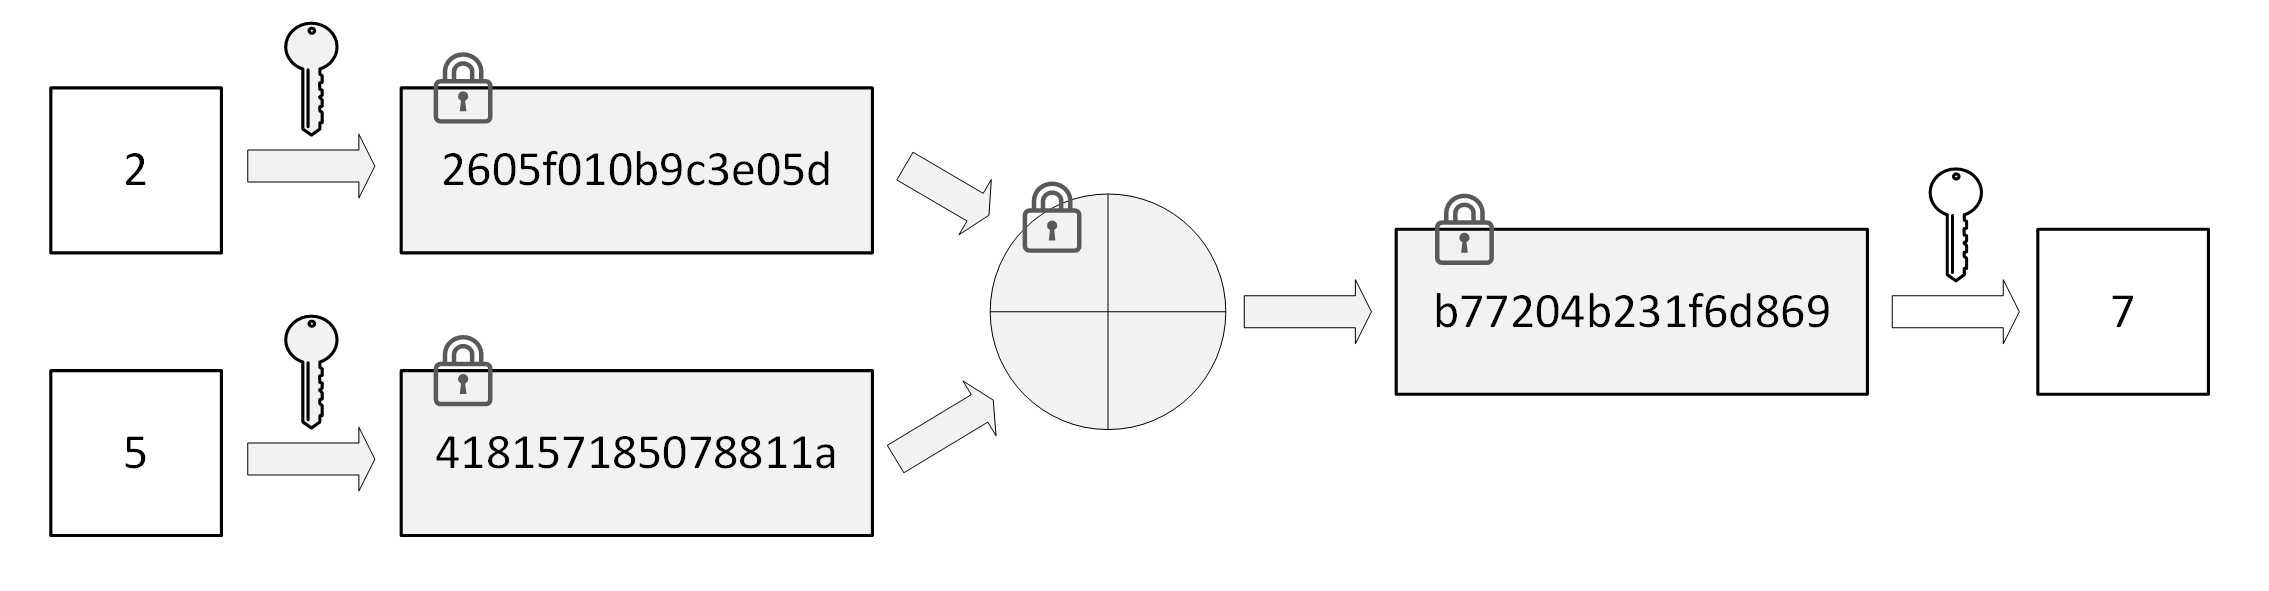
\includegraphics[width=\linewidth]{img/he.png}}
% 	\caption{Example of a homomorphic encryption operation directly on encrypted data. Gray shade indicates public key and encrypted data, while white shade represents plaintexts and secret key.}
% 	\label{fig:he}
% \end{figure}

\subsection{Data-oblivious programming}

{\it Data-oblivious computation} is a type of computation where the input data does not influence the behavior of the program. Under ``behavior'' we imply execution branching or memory access. 
Operations performed on encrypted data have to be in a data-oblivious form since ciphertexts are never decrypted, therefore the program is not capable of making decisions based on their plaintext values. In some fields, this property is also termed as {\it constant-time programming}, and has also been used for protecting against side-channel analysis.

% Consider a simple function calculating Fibonacci numbers in Listing~\ref{list:fibo}

Consider a simple function in Listing~\ref{list:fibo}. The iterations are interrupted once the index {\tt i} reaches the input value \texttt{in}. Assume that computation is now protected so the inputs and outputs must remain encrypted. Since variable {\tt in} cannot participate in any decisions to interrupt iterations, it must be processed in a data-oblivious way. We replace the interrupt condition with a multiplexer accumulator {\tt r} and introduce a fixed number of iterations {\tt max\_iter} not depending on the input, as shown in Listing~\ref{list:fibdo}. The number of iterations should exceed the input index, otherwise the accumulator will not reach the input index and will not get updated. The program shown in Listing~\ref{list:fibdo} works in constant time regardless of the input.

% To do that, we replace the interrupt condition with a multiplexer accumulator
% In this case, the number of iterations should exceed the input index,
\begin{figure}
%\scriptsize
\begin{minipage}{\linewidth}
\begin{lstlisting}[language=C++, caption={Simple Fibonacci function.
% \hspace{1cm} \mbox{}
}, style=mystyle, label=list:fibo, 
% xrightmargin=-0.12\linewidth,
% linewidth=0.96\linewidth
]
int fibonacci(int in)
{
    int i=0, a=0, b=1;
    while( i++ != in )
    {
        std::swap(a,b);
        a += b;
    }
    return a;
}
\end{lstlisting}
\end{minipage}
% \vspace{\lstbspace}
\vspace{-0.1in}
\end{figure}

\begin{figure}
%\scriptsize
\begin{minipage}{\linewidth}
\begin{lstlisting}[language=C++, caption={Data-oblivious Fibonacci function.
% \hspace{-0.05cm} \mbox{}
}, style=mystyle, label=list:fibdo,
% xrightmargin=-0.12\linewidth,
%linewidth=0.96\linewidth
]
int fibonacci(int in)
{
    int i=0, a=0, b=1;
    int r=0;
    int max_iter = 10;
    while( max_iter-- )
    {
        r += (i++ == in) * a;
        std::swap(a,b);
        a += b;
    }
    return r;
}
\end{lstlisting}
\end{minipage}
% \vspace{\lstbspace}
\vspace{-0.2in}
\end{figure}


Changing a program to its data-oblivious form is not trivial. This unavoidable requirement reflects the fundamental property of computation where data is never decrypted, which is the case for all FHE computation. This constraint can affect usability, as existing algorithms may need modifications to be converted to a data-oblivious version.\footnote{Computer-assisted program transformation to data-oblivious variants is an active topic of research, focusing currently on domain-specific languages and compilers \cite{alchemy,fact}.} 
Moreover, it affects practicality too, as fixed iteration upper bounds, introduce performance degradation.

% Moreover, it affects practicality too, as fixed iteration upper bounds, as shown in the example above, introduce performance degradation.

% \subsection{FHE schemes}\label{ss:fheschemes}

% Since the discovery of Fully Homomorphic Encryption~\cite{gentry2009thesis}, various FHE schemes have been released, each focusing on improving different features and functionalities. Popular schemes include BGV (Brakerski-Gentry-Vaikuntanathan) \cite{BGV_ref}, BFV (Brakerski/Fan-Vercauteren) \cite{brakerski2012fully,fan2012somewhatmisc}, CKKS (Cheon-Kim-Kim-Song) \cite{CKKS_ref, cheon2018bootstrapping}, and GSW (Gentry-Sahai-Waters) \cite{GSW_ref}. 

% \noindent {\bf BGV} is an FHE scheme based on the Ring Learning With Errors (RLWE) problem operating over polynomial rings of the form $\mathbb{Z}[X]/(X^{2^n}+1)$. It is
% naturally leveled meaning that without {\it bootstrapping} it allows evaluating a certain number of additions and multiplications on encrypted data, before a predefined {\it noise budget} is consumed.
% BGV encodes plaintext data as coefficients of a polynomial by defining special rules for polynomial addition, as well as multiplication defined as polynomial multiplication modulo a fixed irreducible polynomial. 
% This scheme requires two special operations to support ciphertext multiplication, namely {\it modulus switching} -- a ciphertext rescaling operation, and {\it relinearization} -- restoring the structure of a ciphertext as two sets of coefficients. 
% Given the ability to add and multiply encrypted data, it is possible to define arbitrary computation using either Boolean circuits (arithmetic modulo~2) or more general arithmetic circuits. 
% To address the noise budget limitation, BGV supports Gentry's bootstrapping theorem, which effectively allows resetting the ciphertext noise by homomorphically evaluating a special noise-refreshing circuit \cite{gentry2009fully}. BGV with bootstrapping support has been implemented in the HElib library \cite{githeli_bootstrap}.

% \noindent {\bf BFV} is the next major FHE scheme that introduces two optimizations for relinearization operations that require smaller key sizes and can enable faster performance. 
% BFV, unlike BGV, supports scale-invariant operations; so it does not require any modulus switching throughout the processing of encrypted data. Moreover, BFV is based on modular arithmetic with addition, subtraction, and multiplication support, and the plaintext modulus is usually a large number ($>2^{16}$) \cite{cryptonets, sealpir}. Like BGV, BFV also supports bootstrapping and can perpetually reduce ciphertext noise during computation. BFV without bootstrapping support has been implemented in Microsoft SEAL \cite{seal} and Palisade \cite{palisade} libraries.

% \noindent {\bf CKKS} is the first FHE cryptosystem for approximate arithmetic over complex numbers. CKKS is also based on RLWE. It encodes plaintext data into polynomials, and its modulus switching corresponds to a rounding operation of the encrypted values. Approximate arithmetic is beneficial for encrypted applications that operate on non-integer values, such as neural networks. CKKS has been implemented as part of HElib, Palisade, and SEAL libraries, as well as in the HEANN library, which is specifically developed to support fixed-point FHE arithmetic~\cite{heaan}.

% \noindent {\bf GSW} introduces another approach, called approximate eigenvector method, where the encryption key is an eigenvector of a ciphertext represented as a matrix. This approach enables defining a LWE-based cryptosystem that does not require expensive relinearization operations, and still supports bootstrapping to allow unlimited additions and multiplications of ciphertexts. GSW is the basis for the TFHE scheme \cite{chillotti2016faster} and the FHEW scheme \cite{ducas2015fhew}, both of which define homomorphic Boolean gates with bootstrapping, and allow processing of any Boolean circuit on FHE encryptions of bits (i.e., bit-level arithmetic).

\subsection{FHE Batching}
The FHE batching technique offers the ability to pack several plaintexts into ``slots'' within a single ciphertext. This feature is supported by some FHE schemes, and in practice  enables parallel processing of plaintexts, which are part of the same ciphertext (in a Single Instruction Multiple Data (SIMD) style)~\cite{batching}. Notably, such SIMD processing enables significant performance improvements for algorithms with parallel computation properties.
Each ciphertext variable is effectively a vector of values and any unary or binary operation has the effect of array operations on all elements of these vectors. Using batching, integral data types naturally have arrays of bit values inside each bit of the variable, and gate operations on each separate bit have the effect of the gate operation on all bit values.
BGV, BFV, and CKKS all support batching which enables parallel processing of encrypted vectors of data.

% \vspace{-0.4cm}

% and in practice  enables parallel processing of plaintexts, since they are all part of the same ciphertext